\section{Paramétrisation de l'architecture}

L'architecture à simuler peut être générée à partir de l'architecture réelle de l'utilisateur au moyen d'un fichier XML créé par le logiciel \emph{HWLOC}. Cependant l'utilisateur peut utiliser un fichier de paramétrisation spécifique à notre simulateur qui lui permet d'accéder à l'intégralité des paramètres d'architecture pris en compte.

\subsection{Entrée XML HWLOC}

\emph{HWLOC} est un logiciel libre sous liscence BSD-2. Il permet de générer un fichier XML qui décrit l'architecture de la machine utilisée (commande \verb?lstopo --of xml?). Il décrit notamment la structure arborescente des caches, et donne des informations essentielles pour chaque cache, comme sa taille, la taille de ses lignes et son associativité. 

\paragraph{}
Si l'utilisateur choisit un tel fichier en entrée comme décrivant son architecture, ce dernier sera parsé par une feuille \textit{xslt} en un fichier de configuration de l'architecture personnalisé, comme décrit dans la section \ref{config}. Les paramètres non fournis par le fichier généré par \emph{HWLOC} prendront des valeurs par défaut, proches de celles des architectures \emph{intel} moderne. Cette organisation est décrite par un schéma figure \ref{img:archi}. Notons que notre simulateur ne prend pas en compte les caches de niveau 1 dédiés aux instructions (L1i), qui sont décrits par \emph{HWLOC} mais ne seront pas présent dans le fichier personnalisé.

\begin{figure}[!h]
\begin{center}
   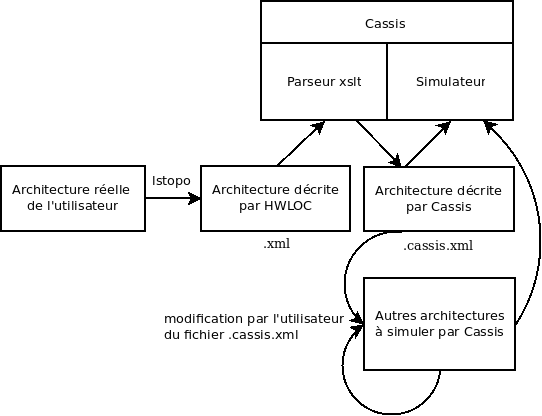
\includegraphics[width=0.7\textwidth]{images/schema_archi.png}
   \caption{\label{img:archi} Fichiers de paramétrisation de l'architecture}
\end{center}
\end{figure}

\subsection{Fichier de configuration personnalisé}
\label{config}
Le fichier de configuration de l'architecture dédié à notre simulateur comprend tous les paramètres d'achitecture utilisables. Une fois généré à partir d'un fichier \emph{HWLOC}, il est possible de l'utiliser directement en entrée du simulateur, après avoir été modifié à la convenance de l'utilisateur. La documentation précise ainsi qu'un exemple de fichier \textit{.cassis.xml} est disponible dans une page de manuel, donnée en annexe \ref{manarchi} page \pageref{manarchi}.

\paragraph{}
Il s'agit d'un fichier XML qui contient 3 balises : \textbf{Architecture}, \textbf{Level} et \textbf{Cache}.

\paragraph{Architecture} donne les infomations générales sur l'architecture, telles que le son nom, le modèle du microprocesseur et le nombre de niveaux de cache.

\paragraph{Level} décrit les informations relatives à un niveau de cache en particulier. Il possède notamment les attributs suivants :
\begin{itemize}
  \item \textbf{coherence\_protocol} : \verb?MESI?, \verb?MSI?, \verb?MOSI?, \verb?MESI? ou \verb?MOESI? (cf. \ref{coherence} page \pageref{coherence}), qui sont les protocoles implémentés pour le simulateur. Le dernier niveau ne possède pas de protocole de cohérence, car il est le seul cache dans son niveau.
  \item \textbf{type} : l'inclusivité des caches du niveau (cf. \ref{inclusivite} page \pageref{inclusivite}). Ce paramètre n'a pas de sens pour les L1.
  \item \textbf{snooping} : y a-t-il du \textit{snooping} à ce niveau ? (cf. \ref{snooping} page \pageref{snooping}). Le cache du dernier niveau ne peut pas faire de \textit{snooping}.
  \item \textbf{directory\_manager} : les caches du niveau possèdent-il un \textit{directory manager} ? Ce paramètre n'est pas pris en compte pour les L1.
\end{itemize}

\paragraph{Cache} concerne les informations spécifiques à un cache en particulier. Il donne notamment la taille en octets du caches, la taille d'une ligne de cache, l'associativité du cache, et enfin le protocole de cohérence du cache(\verb?FIFO?, \verb?LRU? ou \verb?LFU?, cf. \ref{remplacement} page \pageref{remplacement}).

\paragraph{}
Il est ainsi possible de simuler un bon nombre d'architectures, même si certaines n'ont pas de sens. Le simulateur effectue une vérification sur l'achitecture avant la simulation, afin d'écarter certaines architectures qui ont de grandes chances de faire planter le programme. Nous avons néanmoins laissé à l'utilisateur la possibilité de passer outre ces vérifications.


